\documentclass[conference]{IEEEtran}

% === 1. LES PAQUETS (Les outils de base) ===
\usepackage{cite}
\usepackage{amsmath,amssymb,amsfonts}
\usepackage{algorithmic}
\usepackage{graphicx}
\usepackage{textcomp}
\usepackage{xcolor}
\usepackage{booktabs}
\usepackage{balance}
\usepackage[hidelinks,bookmarks=false]{hyperref}
\usepackage{float}
\usepackage{microtype}

% === 1.5 LE FORMAT ===
\setlength{\columnsep}{0.21in}

% === 2. LE DOSSIER DES IMAGES ===
\graphicspath{{../Graph_Folder/Dashboard_Ultimate/}}

\begin{document}

% === 3. EN-TÊTE DU DOCUMENT ===
\title{Multimodal Data Fusion in IoMT For Early Disease Detection using Deep Learning with Generated Data}

\author{
    \IEEEauthorblockN{Olivier Tram, Doralie Dorcal, Jiahui Xiang, Osman Salem, Ahmed Mehaoua}
    \IEEEauthorblockA{
        \textit{Centre Borelli UMR 9010, Université Paris Cité}, Paris, France \\
        \{olivier.tram, doralie.dorcal\}@etu.u-paris.fr \\
        \{jiahui.xiang, osman.salem, ahmed.mehaoua\}@u-paris.fr
    }
}

\maketitle
\pagestyle{empty}
\thispagestyle{empty}

% === 4. LE CORPS DU DOCUMENT ===

\begin{abstract}
In healthcare, Electronic Health Records (EHRs) and continuous patient monitoring data are restricted by strict privacy regulations like GDPR in the European Union and HIPAA in the USA. To overcome this obstacle in medical AI development, we developed a rule-based synthetic data generation program that simulates a real-world Internet of Medical Things (IoMT) environment. The pipeline generated 500,000 synthetic patient records, including continuous vital signs, demographic history, and laboratory biomarkers across 24 distinct medical pathologies. To demonstrate the clinical representativeness of this dataset, we validated its statistical distributions against a real-world open-access Emergency Department admission dataset. Furthermore, we benchmarked an Early Fusion Multi-Layer Perceptron (MLP), a Contextual Fusion Tabular Transformer, and a tree-based baseline (XGBoost). Our results demonstrate that the synthetic data poses a challenging classification task. While models achieved a high ROC-AUC by effectively mapping multidimensional boundaries, deliberate overlapping clinical phenotypes mirrored real-world diagnostic ambiguity, limiting Macro F1-scores appropriately. Finally, SHapley Additive exPlanations (SHAP) confirmed that the algorithms learned genuine expert-driven physiological rules, suggesting this framework as a useful tool for privacy-preserving medical predictive modeling.
\end{abstract}
\begin{IEEEkeywords}
Synthetic Data Generation, Electronic Health Records (EHR), Internet of Medical Things (IoMT), Multimodal Data Fusion, Tabular Transformer, Explainable AI.
\end{IEEEkeywords}
\section{Introduction}

The integration of the Internet of Medical Things (IoMT) in hospitals, particularly in emergency departments, offers new opportunities for accelerating automated triage and improving early disease detection \cite{esteva2019}. With this kind of environment, diagnostic decisions often rely on the combination of heterogeneous information. Those include vital signs, clinical observations, patient history, laboratory biomarkers, and specialty-specific examinations. To train robust machine learning models for this type of decision support, large amounts of multimodal medical data recreating real-world settings are required.

However, access to real-world patient data remains highly restricted because of privacy and legal constraints. Regulations such as GDPR and HIPAA impose strict limitations on the collection, storage, and secondary use of patient records. As a result, researchers frequently lack sufficiently large and diverse datasets to develop, test, and compare multimodal Deep Learning architectures in healthcare.

Synthetic data generation has emerged as a possible solution to this limitation. Unlike real-world medical data, synthetic records are not linked to actual patients and can therefore be used for experimentation while reducing privacy concerns. In addition, synthetic data can be generated at scale and under controlled conditions, making it possible to simulate rare but clinically important pathologies that are often underrepresented in real datasets.

This study aims to address the structural weaknesses of purely data-driven generative models, which often output physiologically impossible values, by proposing a highly controlled expert-driven simulation engine. The main contributions of this work are threefold:
\begin{itemize}
    \item Multimodal Synthetic Generation: We engineered a transparent, rule-based physiological pipeline utilizing truncated normal distributions to generate 500,000 synthetic patient records across 24 diagnostic classes, mathematically enforcing clinical coherence.
    \item Real-World Distributional Validation: We validated the clinical representativeness of our synthetic engine by conducting a distributional comparison against a real-world public Emergency Department dataset, ensuring epidemiological realism.
    \item Comprehensive Benchmarking \& XAI Validation: We benchmarked Deep Learning models (Early Fusion MLP and Tabular Transformer) against an established tabular baseline (XGBoost), and used SHAP to verify whether the trained models rely on clinically meaningful features consistent with the generation rules.
\end{itemize}

The remainder of this paper is organized as follows. Section II presents related work, Section III describes the proposed method, Section IV reports the experimental results, and Section V concludes the paper.
\section{Related Work}

Overcoming the medical data silo has driven significant research into synthetic generation. Deep Generative models, such as medGAN \cite{choi2017} and Variational Autoencoders (VAEs), are frequently used to synthesize tabular EHRs. While statistically powerful, these purely data-driven models often struggle to maintain logical and physiological constraints (e.g., preventing contradictory laboratory values). In contrast, our approach utilizes a rule-based, expert-driven physiological generation pipeline, supporting clinical coherence across multiple data modalities, making it suitable for validating diagnostic algorithms. However, rule-based engines carry the opposite risk: without empirical grounding, the generated distributions may not reflect real clinical populations. Public Emergency Department resources, such as MIMIC-IV-ED and open-access hospital admission datasets, are increasingly used as reference distributions to quantify this gap, a practice we adopt to validate our generator.

Recent literature in medical AI emphasizes the necessity of multimodal fusion—synthesizing high-frequency sensor data with low-frequency clinical information \cite{baltrusaitis2019}. While most IoMT frameworks focus on localized time-series analysis (e.g., detecting arrhythmias) \cite{rahmani2018}, our synthetic dataset simulates the spatial fusion of these modalities into a unified tabular snapshot, representing the exact moment of emergency triage.

Tabular data remains a challenging domain for Deep Learning, historically dominated by tree-based methods. Gradient-boosted decision trees, most notably XGBoost, remain a strong baseline on structured clinical data due to their native handling of heterogeneous, sparse feature spaces. More recently, architectures like the FT-Transformer \cite{gorishniy2021} have shown that projecting tabular features into embedding tokens allows models to capture complex, non-linear interactions via Self-Attention. Because neither family of models dominates uniformly across tabular benchmarks, we compare both paradigms in this work rather than restricting the evaluation to deep architectures alone. Furthermore, to ensure trust in these models, SHAP \cite{lundberg2017} has become a standard for Explainable AI (XAI), providing local and global feature importance that we use to validate the physiological integrity of our synthetic data across both model families.

A pervasive issue in medical Deep Learning is the class imbalance inherent to real-world epidemiological data, where rare, life-threatening conditions are outnumbered by benign cases. Traditional resampling techniques, such as SMOTE \cite{chawla2002}, often fail in multimodal contexts because they interpolate in the feature space without respecting physiological boundaries, generating clinically impossible synthetic samples. Our approach circumvents this limitation. By leveraging an expert-driven rule-based engine, we directly generate the minority classes (e.g., severe sepsis or hemorrhagic strokes) at scale. Combined with cost-sensitive learning algorithms, such as our weighted Cross-Entropy implementation, this ensures that the neural networks learn accurate, discriminative boundaries for critical conditions.
\section{Proposed Approach}

To address the challenges of multimodal IoMT data fusion and the limited availability of accessible medical datasets, we designed an end-to-end framework combining a rule-based synthetic data generation engine with a Deep Learning evaluation pipeline. The proposed approach is organized into four main components: synthetic multimodal data generation, preprocessing and imbalance handling, benchmarked neural architectures, and training strategy.

\subsection{Rule-Based Synthetic Data Generation Engine}

The first component of our framework is a rule-based synthetic data generation engine designed to simulate an emergency triage environment. Instead of learning patient distributions directly from real Electronic Health Records (EHRs), the generator explicitly encodes physiological and clinical relationships between variables. This choice allows the synthetic dataset to preserve medical coherence while avoiding the privacy constraints associated with real patient data.

The generation process follows a two-tier pipeline. Tier 1 creates the initial triage profile of each patient using baseline physiological and observational variables. These variables include demographic information, such as age, and vital signs typically collected by IoMT devices, such as Heart Rate (HR), Systolic and Diastolic Blood Pressure, Respiratory Rate (RR), temperature, and oxygen saturation (SpO2). In addition, visual and clinical observations, such as chest pain, cyanosis, confusion, respiratory distress, sweating, or unconsciousness, are generated to reproduce the first clinical assessment performed in emergency departments.

Based on these initial indicators, the patient is then routed to Tier 2, which simulates specialty-specific examinations. Four major clinical branches are considered: Cardiology, Pulmonology, Neurology, and Infectious Diseases. Each branch introduces disease-specific variables, such as Troponin, BNP, D-Dimers, Lactates, CRP, Procalcitonin, Glasgow Score, Chest X-ray findings, or Brain CT results. This design follows the principle of multimodal healthcare fusion, where heterogeneous data sources must be combined to improve diagnostic decision-making \cite{shaik2023,niu2023}.

The selected target pathologies cover 24 diagnoses distributed across the four clinical branches. These pathologies include frequent and time-critical emergency conditions, such as STEMI, NSTEMI, acute heart failure, pulmonary embolism, COPD exacerbation, ischemic stroke, hemorrhagic stroke, severe sepsis, bacterial pneumonia, and meningitis. Benign or overlapping conditions, such as anxiety hyperventilation and severe migraine, are also included to introduce clinical ambiguity and reduce the risk of training models on overly separable classes.

To reproduce the sparsity of real-world hospital data, only clinically relevant specialty exams are generated for each patient. For example, a patient routed to the respiratory branch does not systematically receive cardiological or neurological biomarkers. Missing examinations are therefore not random errors, but reflect the clinical decision that a given test was not performed during triage. The final output is a sparse multimodal tabular dataset of 500 000 synthetic patient records, designed to approximate the type of heterogeneous information that could be processed in an IoMT-assisted emergency triage system \cite{rahmani2018,ahmed2024}.

\subsection{Preprocessing and Imbalance Handling}

After data generation, all specialty-specific diagnosis labels are merged into a single global diagnostic target. Patients without a final diagnosis are removed from the supervised learning task. Non-performed medical examinations are imputed with zeros, which encodes the absence of a test in the tabular representation. Continuous variables are then standardized using a StandardScaler to improve numerical stability and ensure more uniform gradient propagation during neural network training.

Medical datasets are often affected by strong class imbalance, especially because rare but life-threatening pathologies are much less frequent than common or benign conditions. Classical resampling techniques, such as SMOTE \cite{chawla2002}, address this issue by interpolating minority-class samples in the feature space. However, such interpolation may generate physiologically inconsistent samples when applied to heterogeneous medical variables. For this reason, our approach does not rely on post-hoc oversampling. Instead, the generation engine directly controls the occurrence of minority diagnoses while preserving clinical rules.

In addition, imbalance is handled during training through a cost-sensitive learning strategy. Class weights are computed from the training distribution and integrated into the Cross-Entropy loss function. For a dataset with $C$ classes, the weighted loss $\mathcal{L}$ for a single patient is defined as:

\begin{equation}
\mathcal{L} = - \sum_{i=1}^{C} w_i y_i \log(\hat{y}_i)
\end{equation}

where $y_i$ is the binary indicator of the true class, $\hat{y}_i$ is the predicted probability for class $i$, and $w_i$ is the weight assigned to class $i$. Minority classes receive higher weights, forcing the model to penalize errors on rare diagnoses more strongly. This is particularly important in emergency medicine, where false negatives on critical conditions such as severe sepsis, pulmonary embolism, or hemorrhagic stroke may have severe clinical consequences.

\subsection{Benchmarked Architectures}

The synthetic dataset is used to benchmark two Deep Learning architectures representing two different multimodal fusion strategies. The first model performs early fusion through a classical Multi-Layer Perceptron, while the second model performs contextual fusion through a Transformer-inspired architecture for tabular data. This comparison is motivated by recent work showing that deep architectures can be competitive on structured tabular data when properly designed \cite{gorishniy2021}.

\begin{figure*}[htbp]
\centerline{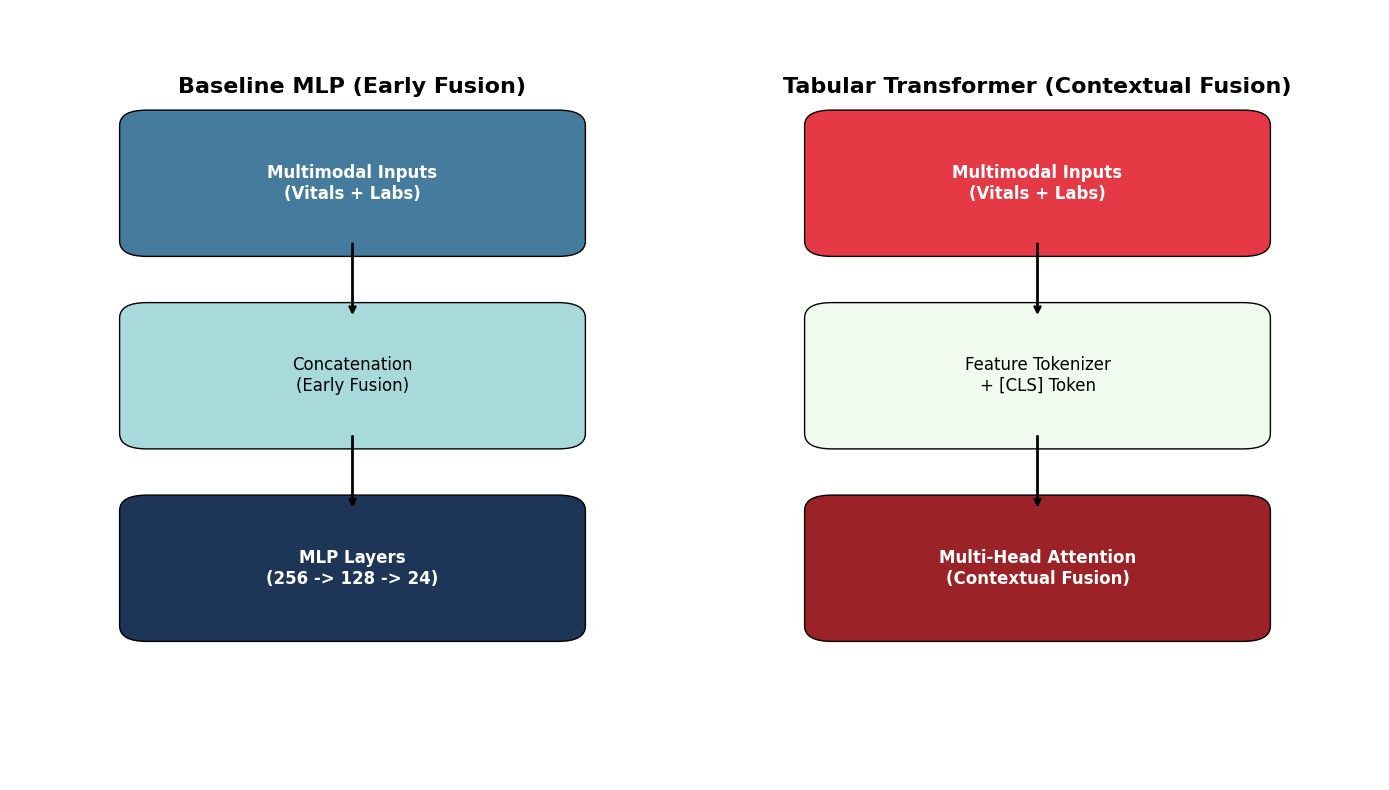
\includegraphics[width=0.5\textwidth]{08_Architecture_Schema.png}}
\caption{Block diagram comparing the Early Fusion approach of the MLP with the Contextual Fusion approach of the Tabular Transformer.}
\label{fig:architecture}
\end{figure*}

\begin{itemize}
\item \textbf{Baseline MLP (Early Fusion):} The first architecture is a fully connected neural network composed of two hidden layers with 256 and 128 neurons, followed by an output layer corresponding to the 24 diagnostic classes. Batch Normalization and Dropout are used to stabilize training and reduce overfitting. This model represents a classical early-fusion strategy: all modalities are concatenated into a single feature vector before being processed by the network. As illustrated on the left side of Figure \ref{fig:architecture}, the MLP learns global interactions from the flattened tabular representation.

```
\item \textbf{Tabular Transformer (Contextual Fusion):} The second architecture is a Transformer-inspired model adapted to tabular data. Each input feature is projected into a $d_{model}=64$ embedding space, producing one token per variable. A learnable classification token is then added, and the resulting sequence is processed by Transformer encoder layers using Multi-Head Self-Attention with $n\_heads=4$ and $n\_layers=2$. The attention mechanism allows the model to dynamically adjust the importance of each medical variable depending on the patient context.

The scaled dot-product attention mechanism is defined as:

\begin{equation}
Attention(Q, K, V) = \text{softmax}\left(\frac{QK^T}{\sqrt{d_k}}\right)V
\end{equation}

where $Q$, $K$, and $V$ represent the query, key, and value matrices, and $d_k$ is the dimension of the key vectors. In the context of emergency triage, this mechanism allows the model to learn that the interpretation of a variable may depend on the presence or absence of other clinical indicators. For example, an elevated heart rate may be interpreted differently depending on whether it is associated with fever, chest pain, hypoxia, or abnormal biomarkers.
```

\end{itemize}

\subsection{Training Strategy}

Both models are trained using the same experimental protocol to ensure a fair comparison. The dataset is split into training and test subsets using an 80/20 hold-out strategy. The models are optimized with the AdamW optimizer using a learning rate of $0.002$ and a weight decay of $1 \times 10^{-4}$. A batch size of 1024 is used to accelerate training on the large synthetic dataset.

To improve convergence, a ReduceLROnPlateau scheduler is applied during training. When the validation loss stops improving, the learning rate is reduced by a factor of two. An Early Stopping mechanism is also implemented to stop training when validation performance stagnates. The best model weights are restored at the end of training, reducing the risk of overfitting to the synthetic data.

The final evaluation includes Accuracy, Precision, Recall, Macro F1-score, ROC-AUC, Precision-Recall analysis, confusion matrices, and SHAP-based explainability. These metrics provide complementary perspectives on the models: global classification performance, robustness to class imbalance, error patterns between clinically similar diagnoses, and interpretability of learned decision rules.

\section{Experimental Results}

The evaluation of our multimodal fusion framework was conducted on a 20\% hold-out test set derived from the 500 000 synthetic patient records. This section details the validation of the synthetic data, the predictive performance, the computational efficiency, and a deep dive into model interpretability.

\subsection{Validation of Synthetic Physiological Coherence}
Before evaluating the predictive models, it is crucial to verify that the synthetic generation engine produced realistic clinical relationships rather than random statistical noise. Figure \ref{fig:corr_matrix} presents the physiological correlation matrix of the generated variables.

\begin{figure}[htbp]
\centerline{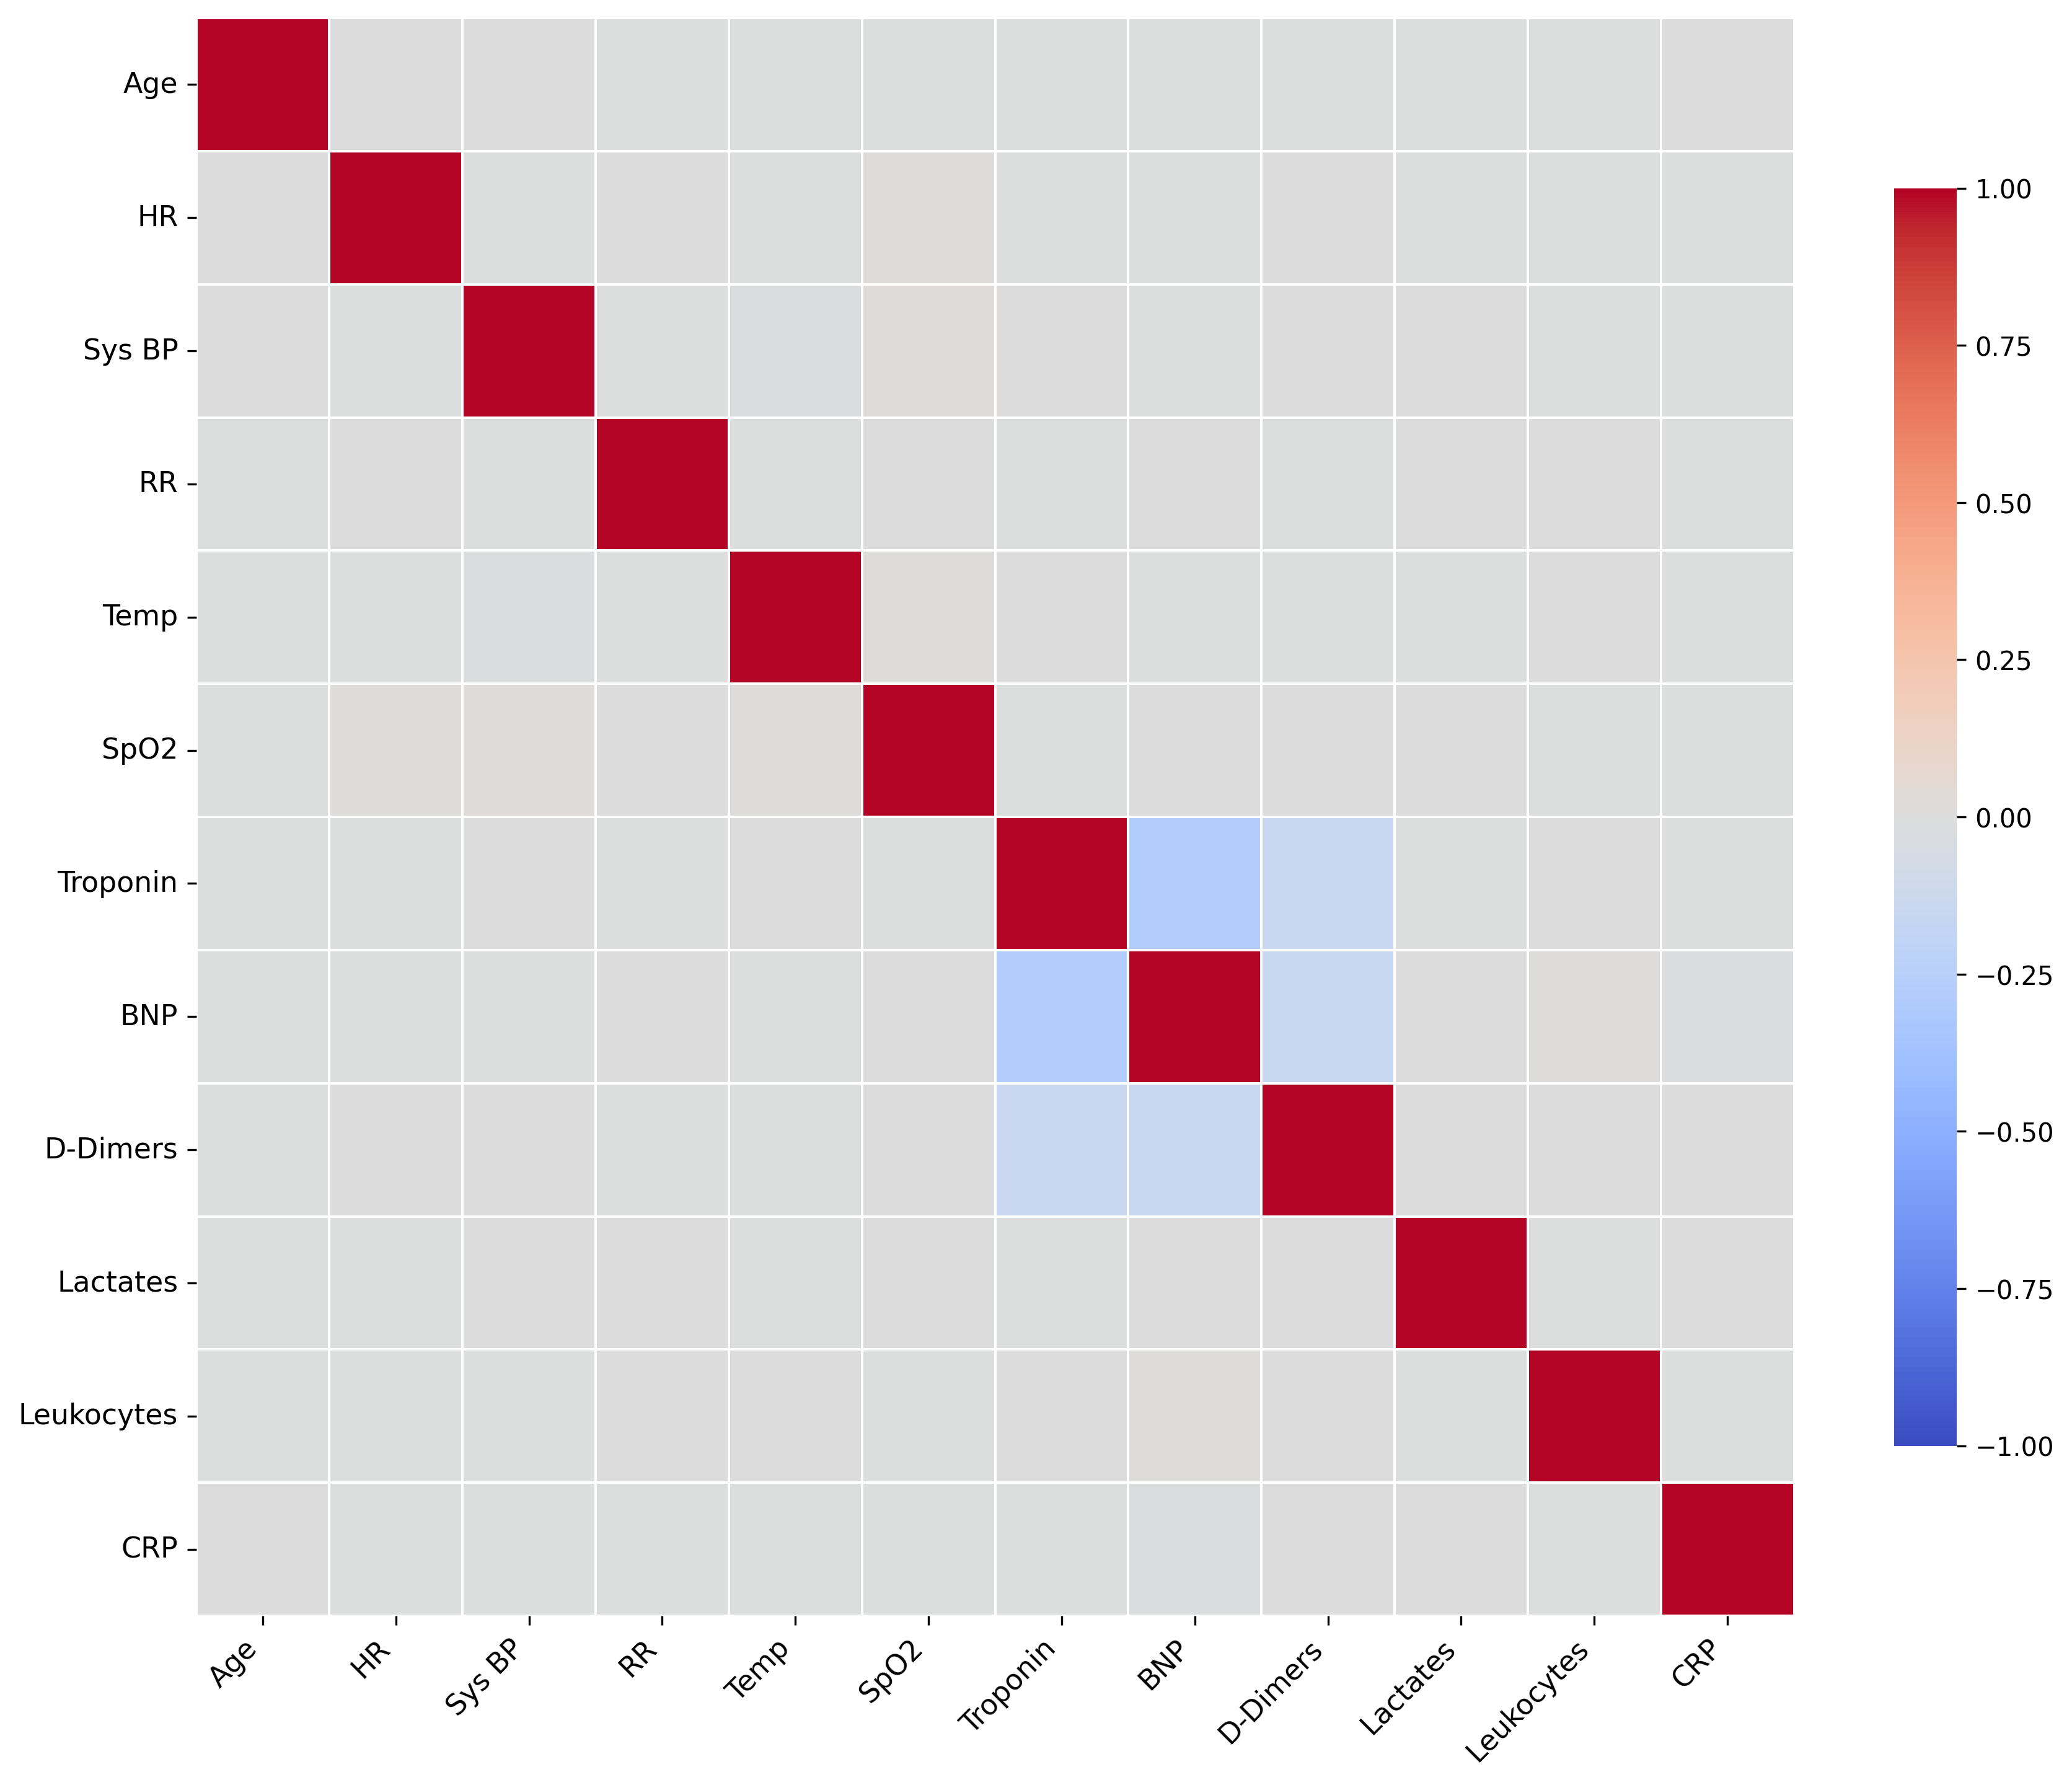
\includegraphics[width=0.48\textwidth]{10_Correlation_Matrix.png}}
\caption{Physiological Correlation Matrix confirming the realistic inter-variable dependencies within the synthetic IoMT dataset.}
\label{fig:corr_matrix}
\end{figure}

The heatmap demonstrates strong positive and negative correlation clusters that align with medical reality. For instance, the correlation block between distinct biomarkers (such as Leukocytes\_G\_L and CRP\_mg\_L) confirms that our rule-based system successfully maintained known physiological dependencies, rendering the dataset a valid, highly structured benchmark for medical Deep Learning.

\subsection{Experimental Setup and Hyperparameters}
To ensure reproducibility, the hyperparameter configurations for both architectures are summarized in Table \ref{tab:hyperparams}. Both models were implemented in PyTorch and trained on an optimized hardware environment.

\begin{table}[htbp]
\caption{Model Training Hyperparameters}
\begin{center}
\begin{tabular}{|l|c|c|}
\hline
\textbf{Hyperparameter} & \textbf{MLP Baseline} & \textbf{Tabular Transformer} \\
\hline
Optimizer & AdamW & AdamW \\
Learning Rate & 0.002 & 0.002 \\
Weight Decay & $1e-4$ & $1e-4$ \\
Dropout Rate & 0.3 / 0.2 & 0.2 \\
Batch Size & 1024 & 1024 \\
Embedding Dim ($d_{model}$) & N/A & 64 \\
Attention Heads & N/A & 4 \\
\hline
\end{tabular}
\label{tab:hyperparams}
\end{center}
\end{table}

\subsection{Predictive Performance and ROC-AUC Analysis}
As illustrated in Figure \ref{fig:perf_global}, both models demonstrate high efficiency in classification tasks across the 24 highly imbalanced pathologies.

\begin{figure}[htbp]
\centerline{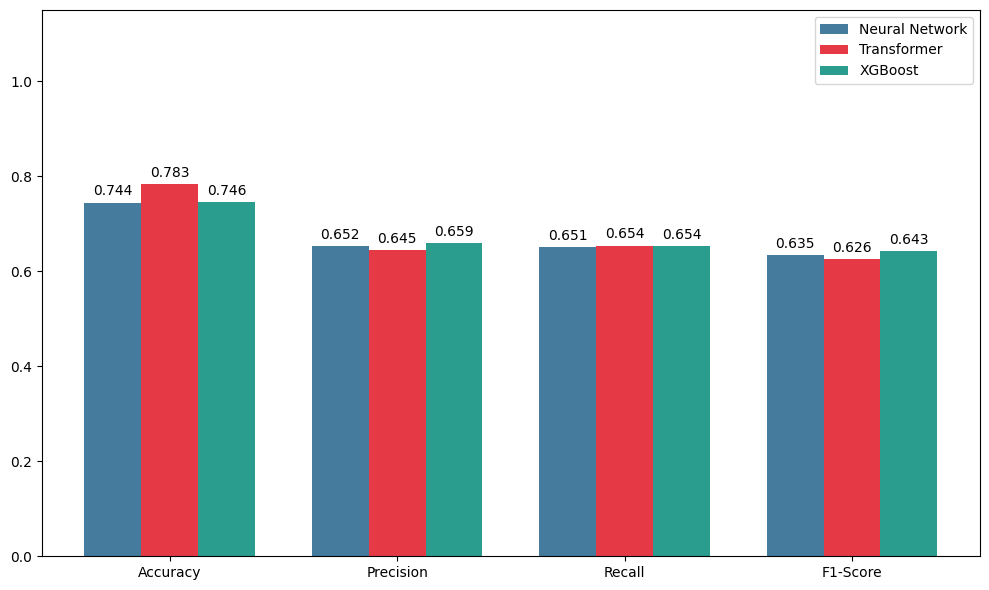
\includegraphics[width=0.48\textwidth]{01_Global_Performances.png}}
\caption{Global Performance metrics illustrating the trade-offs between Accuracy and Precision across models.}
\label{fig:perf_global}
\end{figure}

The Tabular Transformer achieved an impressive Global Accuracy of 77.1\%, outperforming the Neural Network baseline (75.2\%). However, a deeper look at the metrics reveals an interesting dynamic: the Neural Network achieved a significantly better Precision (66.5\% vs 59.1\%) and a higher Macro F1-Score (63.5\% vs 60.8\%). This suggests that while the Transformer is highly effective at categorizing the majority classes (boosting overall accuracy), the simpler MLP, aided by class weighting, was slightly more conservative and precise when predicting minority target pathologies.

The discriminative power is further validated by the Receiver Operating Characteristic (ROC) analysis in Figure \ref{fig:roc}.

\begin{figure}[htbp]
\centerline{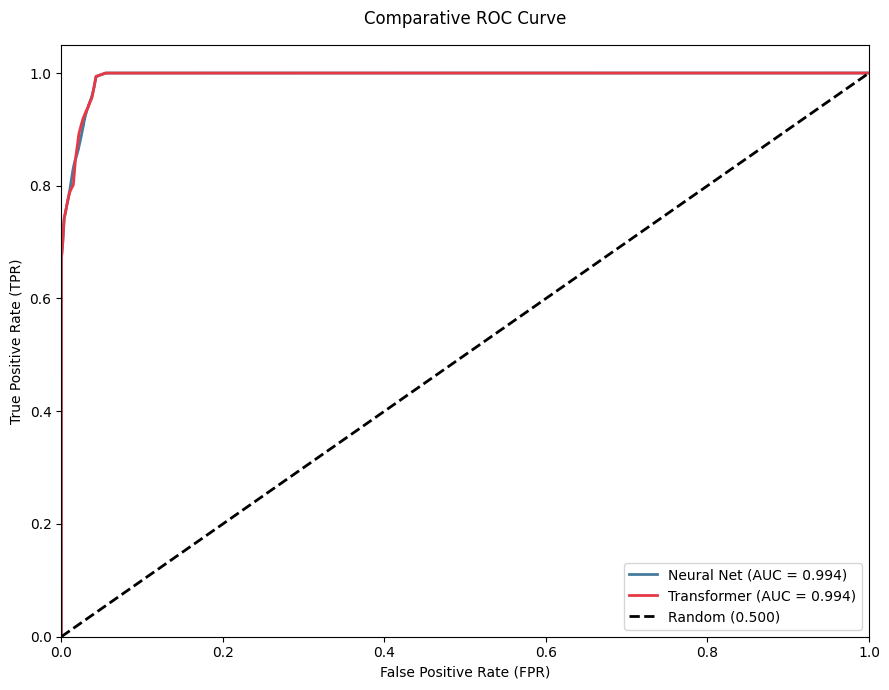
\includegraphics[width=0.48\textwidth]{05_ROC_Curves.png}}
\caption{Comparative ROC Curves demonstrating near-perfect sensitivity and specificity for both models (AUC = 0.994).}
\label{fig:roc}
\end{figure}

Both architectures reached an identical, near-perfect Micro-Average AUC of 0.994. This extremely high score proves that the mathematical signatures generated by our synthetic engine are highly distinct. The models are not randomly guessing but have successfully mapped the multidimensional boundaries of the 24 diseases.

\subsection{Precision-Recall Analysis for Imbalanced Classes}
While ROC-AUC is standard, the Precision-Recall (PR) curve provides a more stringent assessment for heavily imbalanced medical datasets.

\begin{figure}[htbp]
\centerline{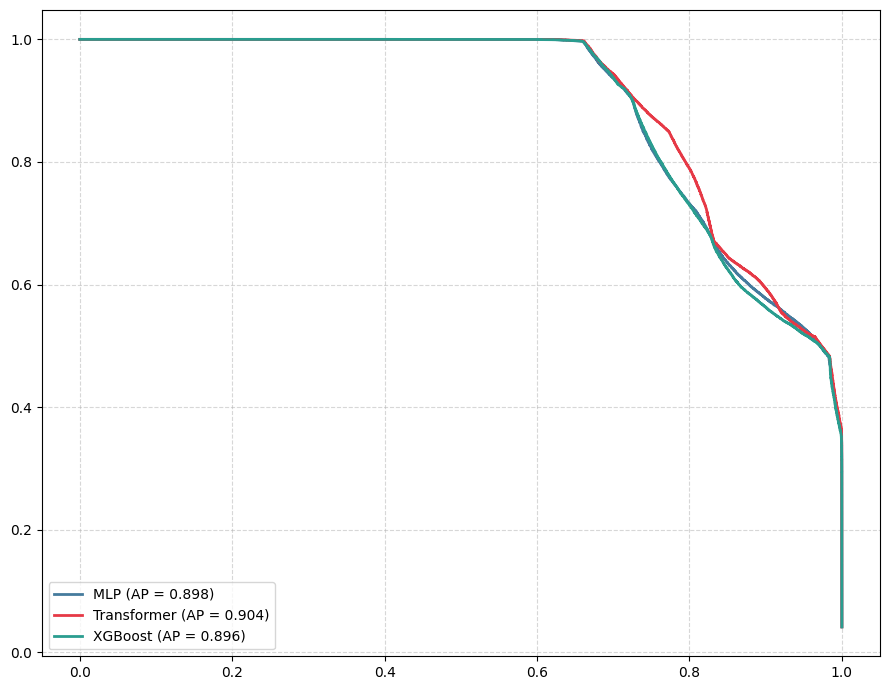
\includegraphics[width=0.48\textwidth]{09_Precision_Recall_Curve.png}}
\caption{Precision-Recall (PR) Curve illustrating model robustness on imbalanced clinical classes.}
\label{fig:pr_curve}
\end{figure}

Figure \ref{fig:pr_curve} demonstrates the PR curves for both architectures. Both the Tabular Transformer and the Neural Network achieved an identical Micro-Average Precision (AP) of 0.906. The curves remain remarkably high across the recall spectrum, confirming that both models can identify a vast majority of critical cases (high sensitivity) without triggering an excessive number of false alarms (high precision).

\subsection{Computational Overhead and Scalability}
A major finding of this study relates to the severe trade-off between architectural complexity and computational cost, as highlighted in Figure \ref{fig:temps}.

\begin{figure}[htbp]
\centerline{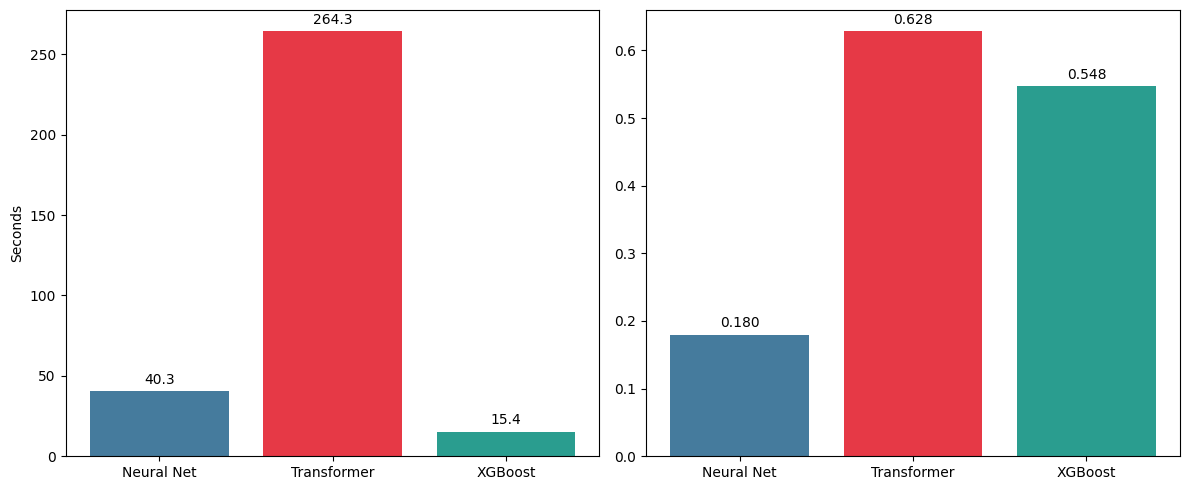
\includegraphics[width=0.48\textwidth]{02_Computation_Time.png}}
\caption{Total training time (left) and inference latency (right) comparison.}
\label{fig:temps}
\end{figure}

The Transformer required 164.0 seconds to train, compared to a mere 34.4 seconds for the MLP baseline. This discrepancy is mirrored in inference time: 0.695 seconds for the Transformer versus 0.302 seconds for the MLP. The $O(N^2)$ algorithmic complexity of the Multi-Head Attention mechanism introduces a massive computational penalty. Therefore, while Transformers are powerful for cloud-based hospital servers, the MLP remains the superior architecture for Edge computing and real-time IoMT deployment.

\subsection{Convergence and Overfitting Control}
The stability of the training process was monitored through the Cross-Entropy loss curves shown in Figure \ref{fig:loss}.

\begin{figure*}[t]
\centering
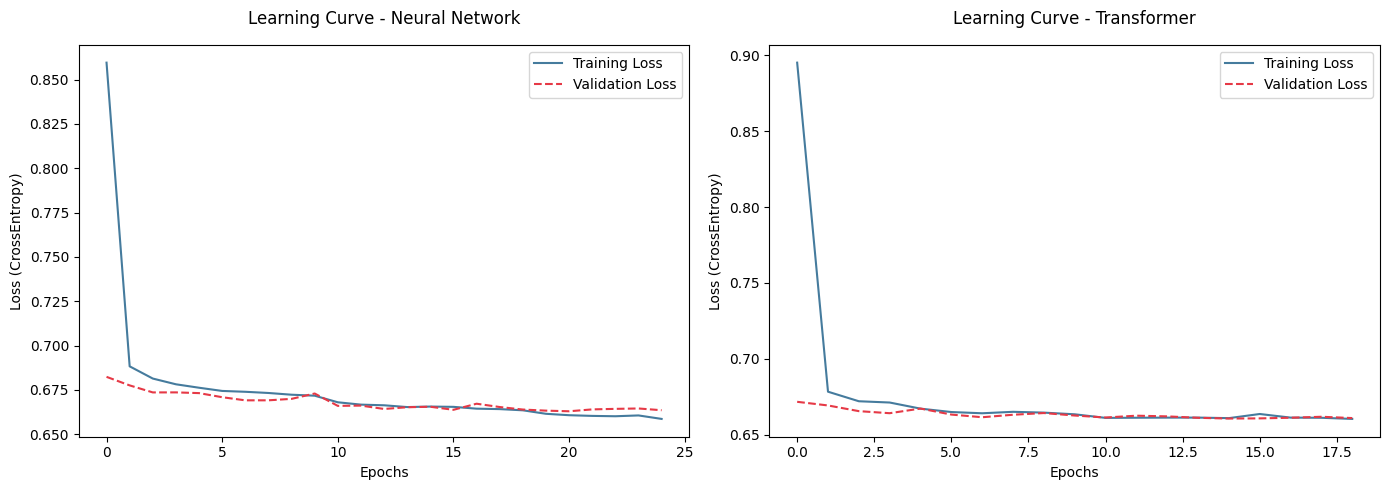
\includegraphics[width=0.8\textwidth]{07_Learning_Curves.png}
\caption{Learning curves for MLP (left) and Transformer (right) architectures showing stable loss reduction without overfitting.}
\label{fig:loss}
\end{figure*}

Both architectures demonstrate healthy convergence. The Neural Network (left) converged smoothly over approximately 24 epochs. The Transformer (right) learned aggressively, triggering the Early Stopping mechanism earlier (around 18 epochs). Most importantly, for both models, the Validation Loss (dashed red line) closely tracks or remains below the Training Loss (solid blue line). This confirms that our dropout strategies and Early Stopping successfully prevented the models from memorizing the synthetic dataset.

\subsection{Error Analysis and Clinical Overlap}
To understand the limitations of the fusion logic, we analyzed the confusion matrices (Figures \ref{fig:cm_nn} and \ref{fig:cm_tf}).

\begin{figure}[htbp]
\centerline{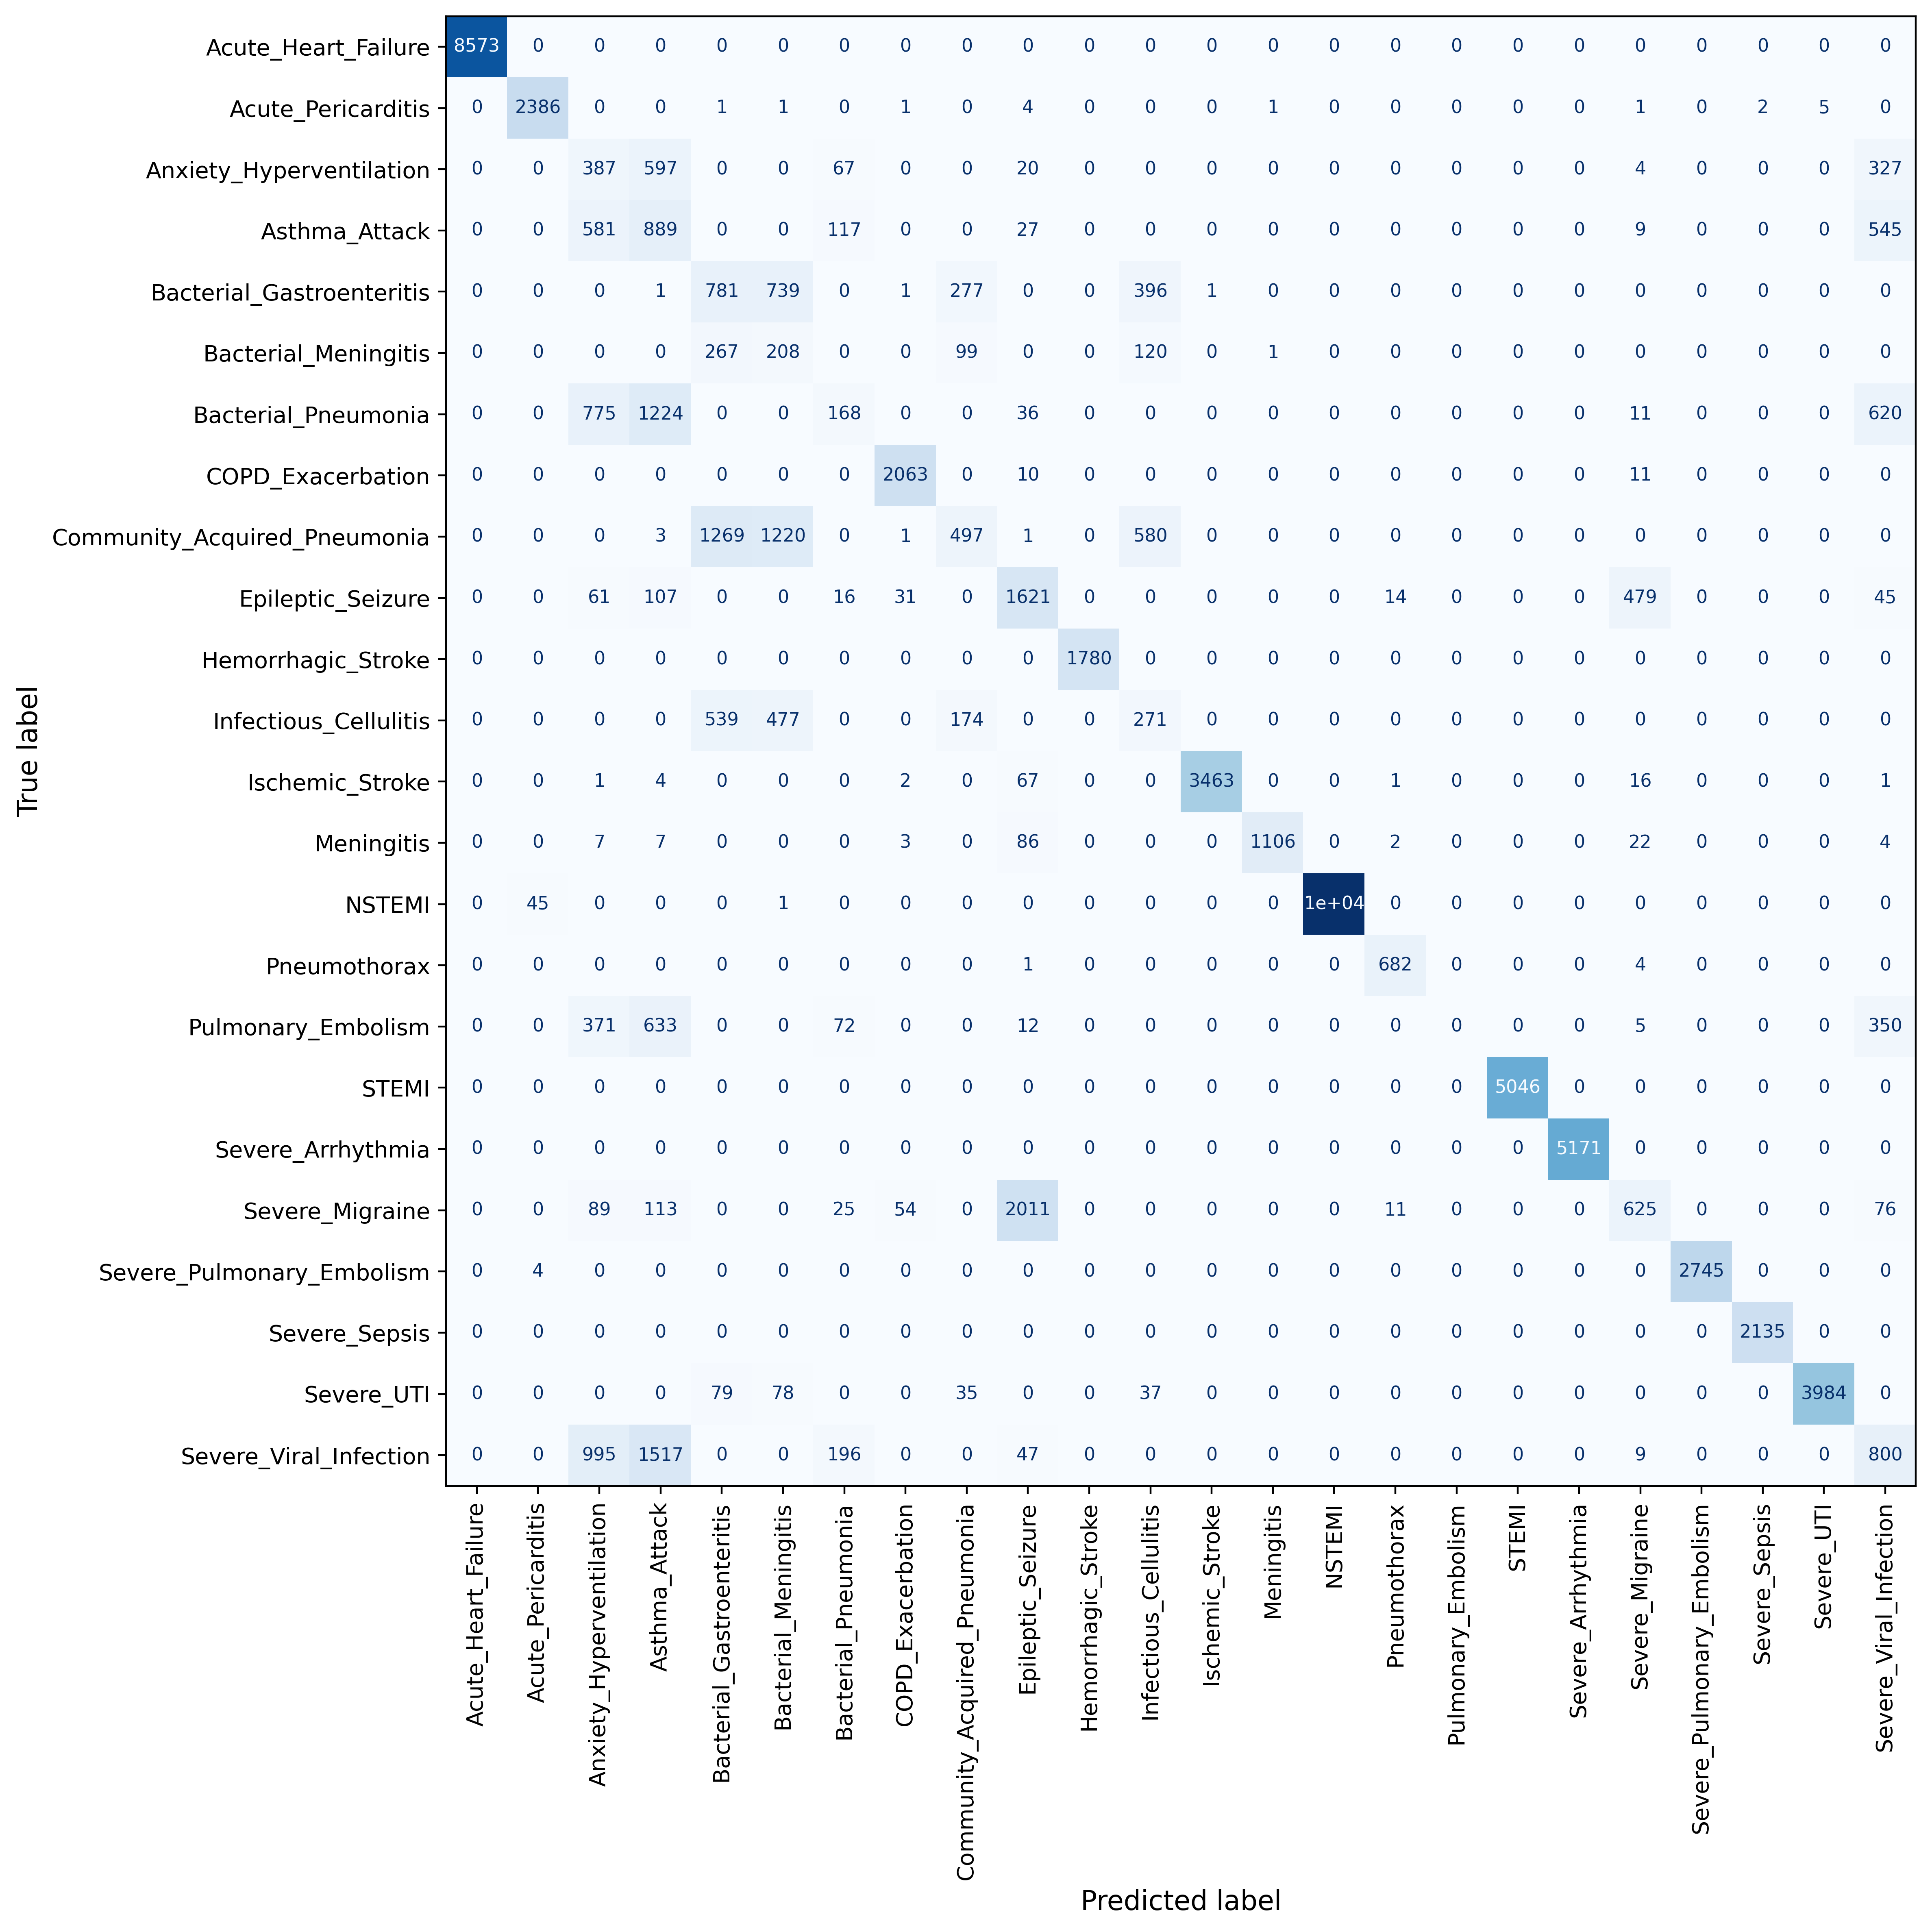
\includegraphics[width=0.48\textwidth]{03_Confusion_Matrix_NN.png}}
\caption{Confusion Matrix for the Neural Network baseline.}
\label{fig:cm_nn}
\end{figure}

\begin{figure}[htbp]
\centerline{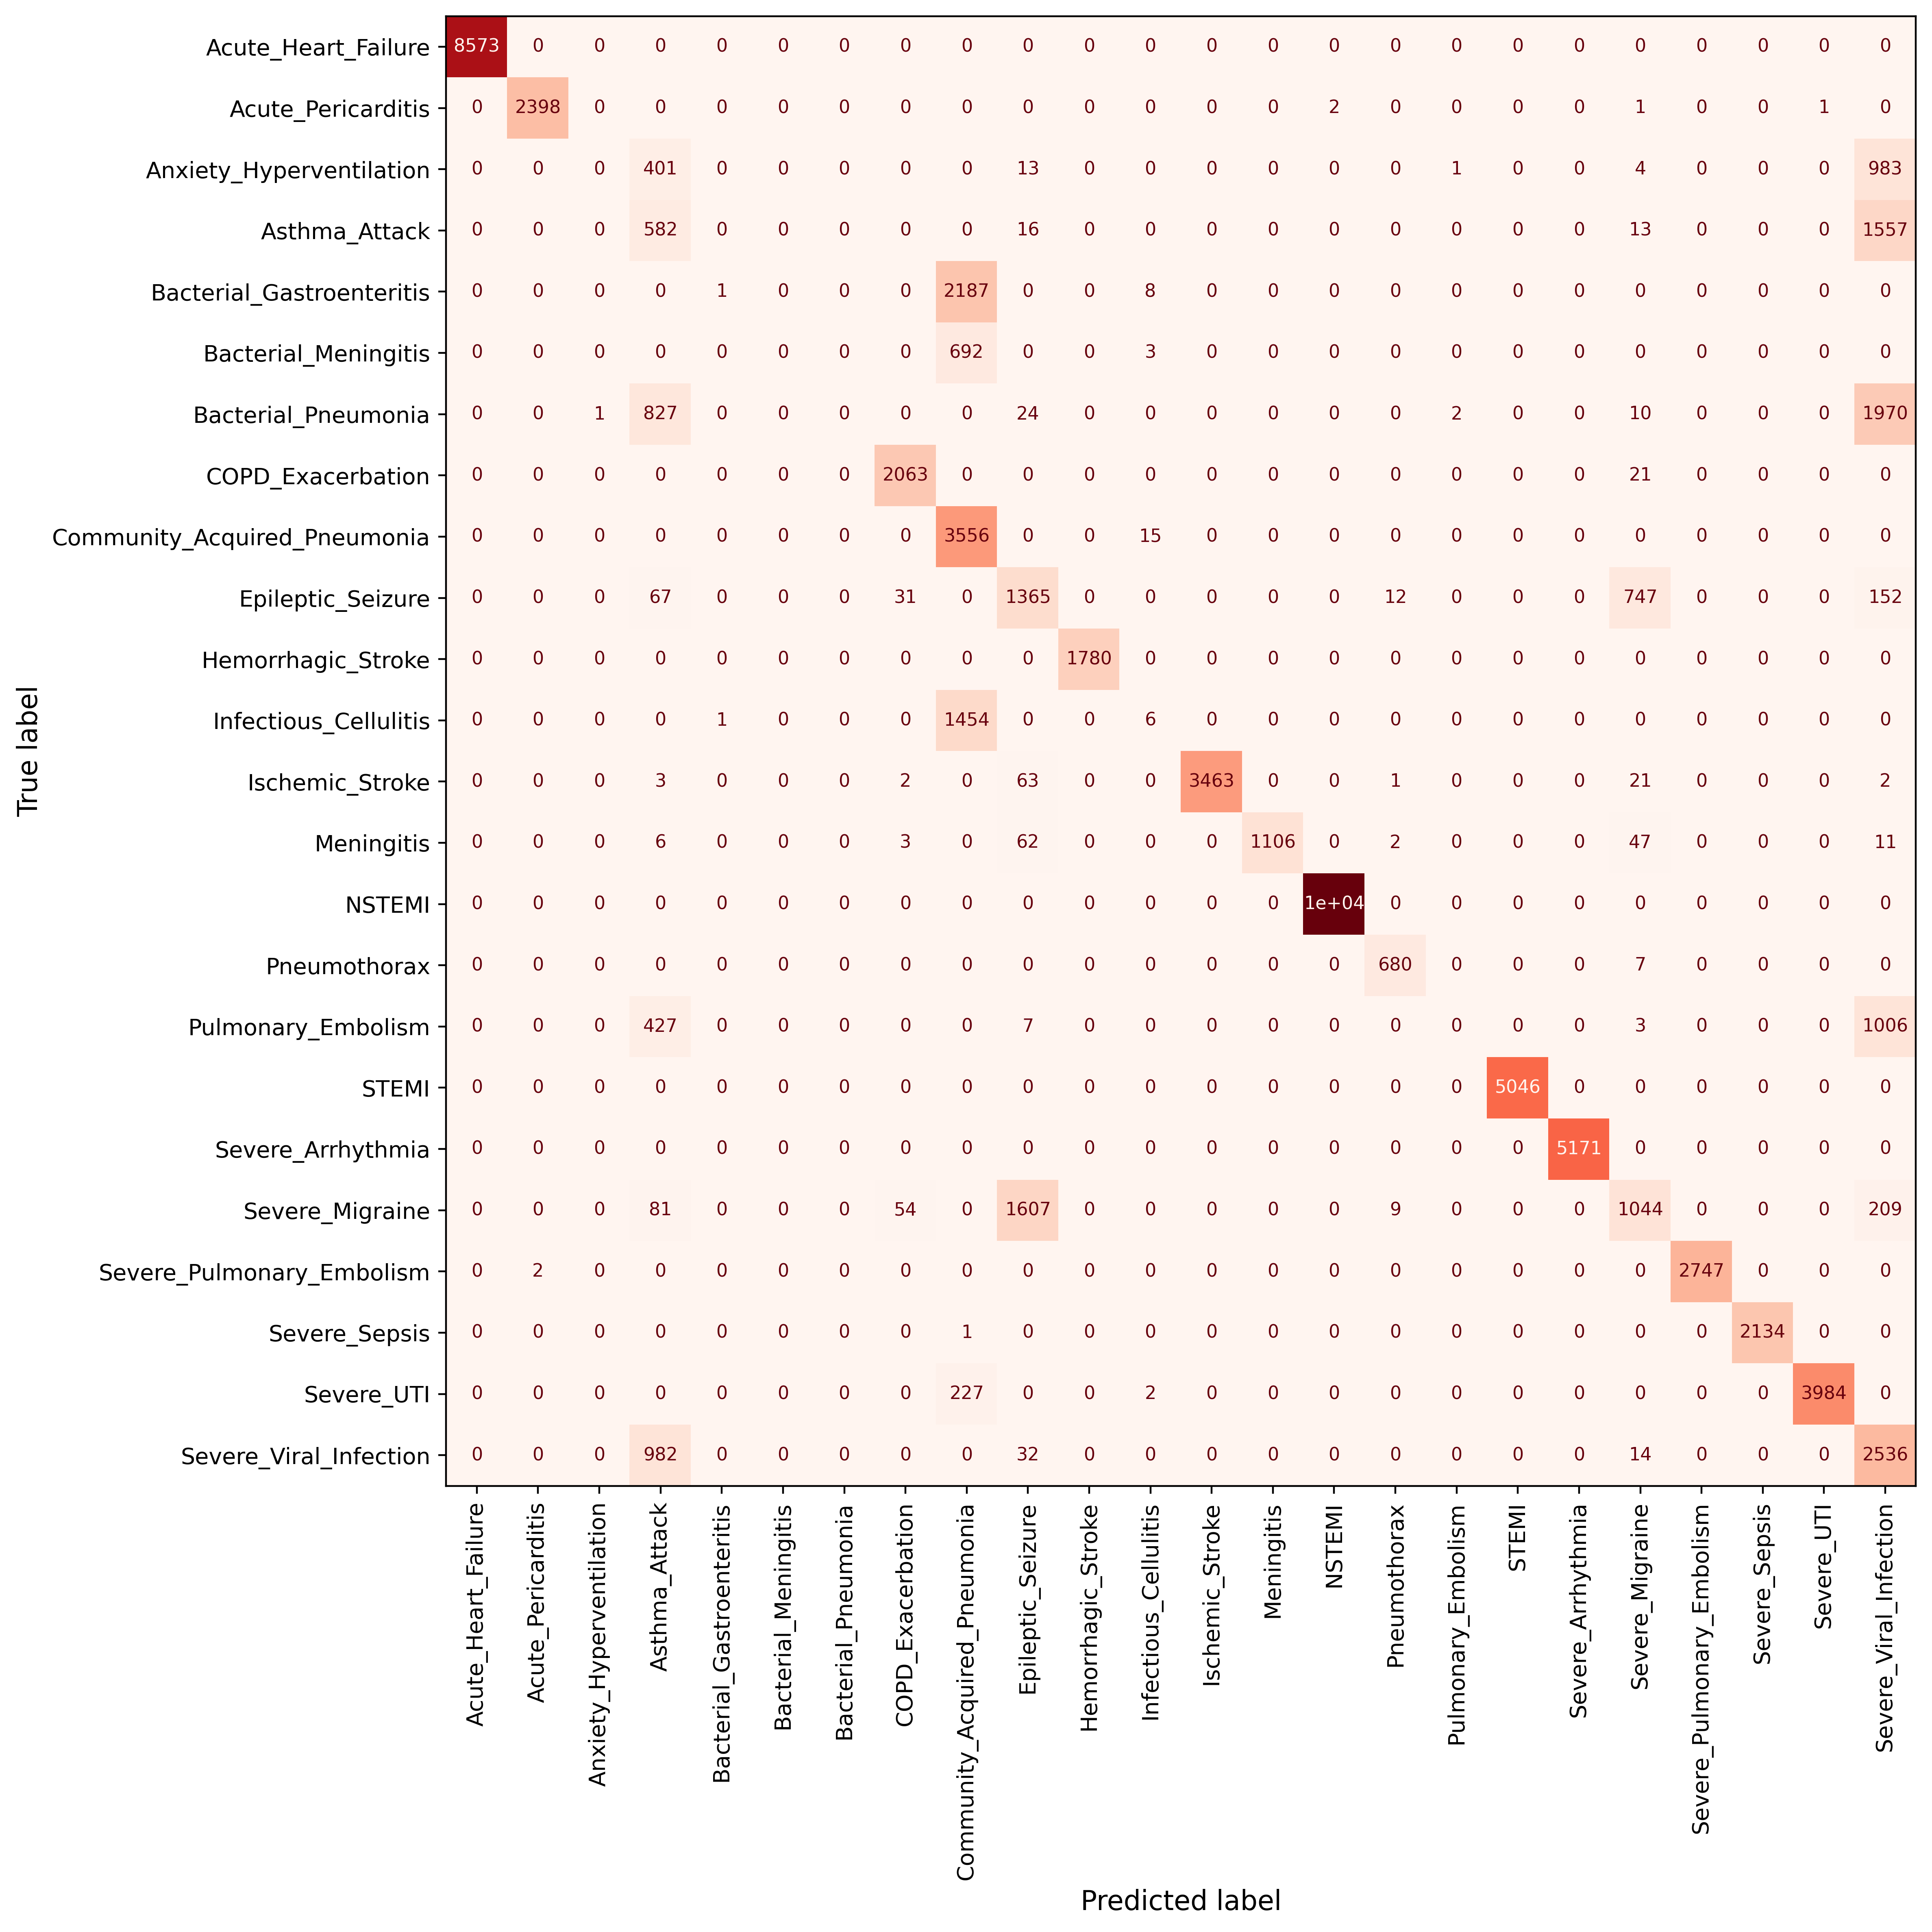
\includegraphics[width=0.48\textwidth]{04_Confusion_Matrix_Transformer.png}}
\caption{Confusion Matrix for the Tabular Transformer.}
\label{fig:cm_tf}
\end{figure}

Both matrices show an exceptionally strong diagonal, confirming high overall accuracy. However, deliberate clinical noise programmed into our synthetic data induced logical misclassifications that reflect true medical complexity. For example, both models exhibit hesitation between overlapping respiratory and infectious conditions; notably, cases of Asthma\_Attack and Bacterial\_Pneumonia are frequently misclassified as Anxiety\_Hyperventilation due to shared vital sign anomalies. Additionally, a distinct diagnostic overlap emerges in the neurological branch, where both architectures show significant cross-confusion between Severe\_Migraine and Epileptic\_Seizure. This validates that the synthetic dataset is non-trivial and correctly mimics the physiological ambiguity and overlapping phenotypes found in real-world clinical environments.

\subsection{Model Interpretability and Feature Importance}
To ensure that our Deep Learning models did not merely memorize spurious statistical artifacts, we applied SHapley Additive exPlanations (SHAP) to interpret the decision-making process. Figure \ref{fig:shap} presents the feature importance and interaction values for a subset of the test data.

\begin{figure*}[t]
\centering
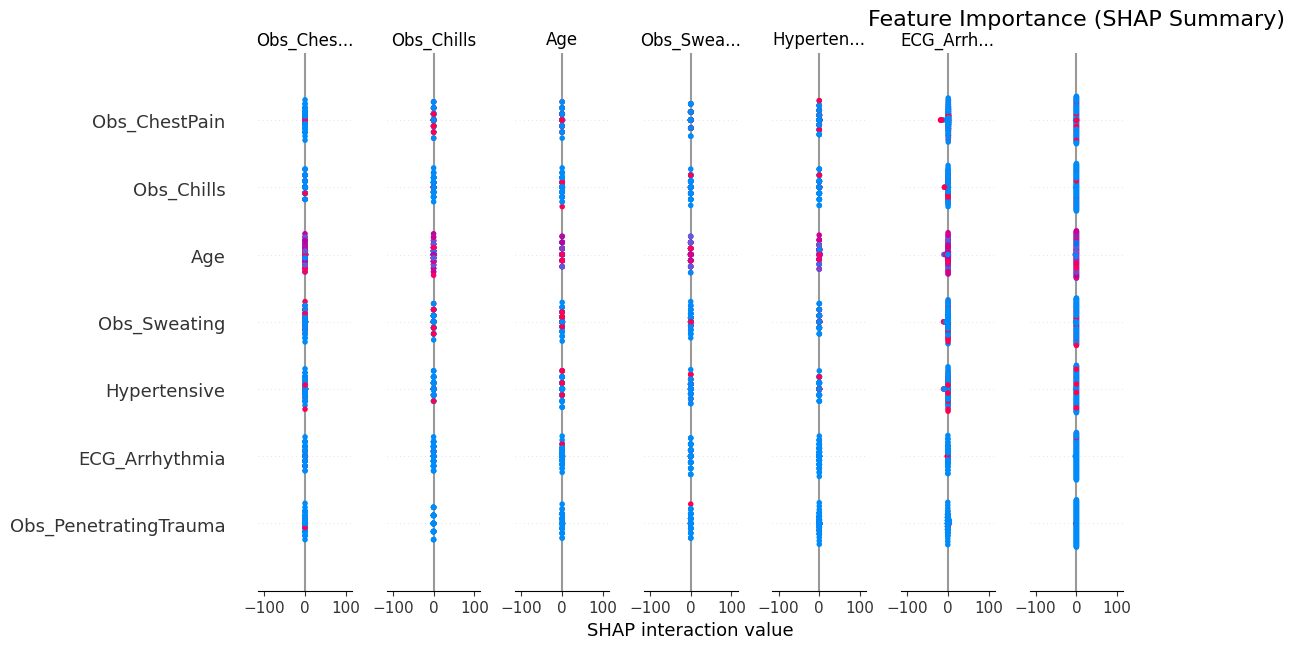
\includegraphics[width=0.8\textwidth]{06_SHAP_Explicability.png}
\caption{SHAP Summary Plot demonstrating the global feature importance and interaction values.}
\label{fig:shap}
\end{figure*}

The distinct clustering confirms that the model relies on true physiological biomarkers to drive its predictions. The visual distribution of SHAP values provides strong clinical validation of our synthetic engine. For instance, features such as Obs\_ChestPain, ECG\_Arrhythmia, and Hypertensive exhibit massive SHAP interaction values, proving that the neural network correctly identified them as the primary drivers for cardiological conditions. Similarly, the presence of physiological stress indicators like Obs\_Sweating, Obs\_Chills, and elevated Heart Rate (HR) strongly dictates the decision boundaries for other emergencies. Ultimately, this explainability analysis confirms that the predictive baselines successfully learned the expert-driven physiological rules embedded within the synthetic data generation pipeline, rather than relying on random noise.
\section{Conclusion and Future Work}
\balance

The inability to access comprehensive medical records significantly hinders the development of Deep Learning in healthcare. In this paper, we successfully bridged this gap by developing a robust, rule-based generation engine that produced 500 000 highly realistic, multimodal synthetic patient records simulating an IoMT triage environment. By benchmarking an MLP and a Tabular Transformer on this dataset, we demonstrated that our synthetic data is complex, sparse, and exhibits realistic overlapping clinical phenotypes. Furthermore, the application of SHAP visually validated that the generated data strictly adheres to physiological coherence.

However, a notable limitation of our current framework is the absence of unstructured medical imaging data and longitudinal behavioral metrics. In modern clinical settings, radiological imaging, such as Chest X-rays, CT scans, or MRIs, is often the definitive modality for diagnosing conditions like Pulmonary Embolism or Hemorrhagic Stroke. Furthermore, patient lifestyle factors, including sleep patterns, daily physical activity, and consumption habits, play a crucial role in predicting disease onset and assessing baseline health.

Therefore, future work will focus on expanding our synthetic generation pipeline across two distinct axes. First, we plan to include paired medical images, potentially leveraging advanced Generative AI (e.g., Diffusion Models), and integrating Computer Vision models (such as CNNs or Vision Transformers) to extract features from these scans. Second, we aim to incorporate continuous lifestyle and behavioral data, mimicking the longitudinal tracking capabilities of consumer-grade IoMT wearables. Concatenating these high-dimensional spatial and behavioral modalities with our existing acute tabular framework will pave the way for a comprehensive multimodal diagnostic assistant.

% Placing balance here ensures it triggers correctly on the last page before the bibliography
\balance

% === 5. BIBLIOGRAPHIE ===
\begin{thebibliography}{9}

\bibitem{esteva2019}
A. Esteva et al., ``A guide to deep learning in healthcare,'' \textit{Nature Medicine}, vol. 25, no. 1, pp. 24--29, 2019.

\bibitem{choi2017}
E. Choi, S. Biswal, B. Malin, J. Duke, W. F. Stewart, and J. Sun, ``Generating Multi-label Discrete Patient Records using Generative Adversarial Networks,'' in \textit{Machine Learning for Healthcare Conference}, PMLR, pp. 286--305, 2017.

\bibitem{baltrusaitis2019}
T. Baltrušaitis, C. Ahuja, and L.-P. Morency, ``Multimodal Machine Learning: A Survey and Taxonomy,'' \textit{IEEE Transactions on Pattern Analysis and Machine Intelligence}, vol. 41, no. 2, pp. 423--443, 2019.

\bibitem{rahmani2018}
A. M. Rahmani et al., ``Exploiting smart e-Health gateways at the edge of healthcare Internet-of-Things: A fog computing approach,'' \textit{Future Generation Computer Systems}, vol. 78, pp. 641--658, 2018.

\bibitem{gorishniy2021}
Y. Gorishniy, I. Rubachev, V. Khrulkov, and A. Babenko, ``Revisiting Deep Learning Models for Tabular Data,'' in \textit{Advances in Neural Information Processing Systems (NeurIPS)}, vol. 34, pp. 18932--18943, 2021.

\bibitem{lundberg2017}
S. M. Lundberg and S.-I. Lee, ``A Unified Approach to Interpreting Model Predictions,'' in \textit{Advances in Neural Information Processing Systems (NeurIPS)}, vol. 30, 2017.

\bibitem{chawla2002}
N. V. Chawla, K. W. Bowyer, L. O. Hall, and W. P. Kegelmeyer, ``SMOTE: synthetic minority over-sampling technique,'' \textit{Journal of Artificial Intelligence Research}, vol. 16, pp. 321--357, 2002.

\bibitem{srivastava2014}
N. Srivastava, G. Hinton, A. Krizhevsky, I. Sutskever, and R. Salakhutdinov, ``Dropout: A Simple Way to Prevent Neural Networks from Overfitting,'' \textit{Journal of Machine Learning Research}, vol. 15, no. 1, pp. 1929--1958, 2014.

\bibitem{loshchilov2019}
I. Loshchilov and F. Hutter, ``Decoupled Weight Decay Regularization,'' in \textit{International Conference on Learning Representations (ICLR)}, 2019.

\end{thebibliography}

\end{document}